\chapter{Context and objectives} \label{chapter2}
\minitoc
\eject

\section{Introduction}

This chapter presents the general context for this work, and leads to a definition of the problematic addressed in this thesis.
Section \ref{chapter2:web-as-a-platform} presents the context for the web development, and the motivation that led the web to become a software platform. It presents briefly the main languages available for initiating a web application, and a great section is dedicated to Javascript, as it is increasingly gained popularity these past few years.
Section \ref{chapter2:highly-concurrent-web-servers} presents the problematic for developping web server for large audiences.
It explains why the languages presented in the previous section often fail to grow with the project they initially supported very efficiently.
It conclude that this rupture is an economical risk for young projects.
Finally, section \ref{chapter2:equivalence} presents the goal of this work.
That is to reconcile the technologies used in the initial phase of a project, with the ones used to grow the project in performance.

\section{The Web as a platform}

\subsection{From operating systems to the web}


With the invention of electronic computing machine, appeared the market for software applications.
This market is not limited by marginal production cost ; software being a virtual product, the production and distribution cost for another unit is virtually null.
The market is limited by the platform a software can be deployed on.
The bigger the platform, the wider the market.
There is an economically incentive to standardize and widen the platform, both for the provider, and for the consumer.
The first platforms started as products, in competition with other products.
Their manufacturers had economical incentive to increase their market share.
Microsoft successfully took over the market of operating system in the 90s, and was on the edge of monopoly more than once.
But eventually, the product is standardized, and becomes the platform.

\begin{wrapfigure}{r}{0.2\textwidth}
  \vspace{-27pt}
  \begin{center}
    \includegraphics[width=0.18\textwidth]{../ressources/Mac-PC.png}
  \end{center}
  \vspace{-20pt}
\end{wrapfigure}

Before the internet, this market was limited for distribution by the physical medium.
It takes time to burn a CD, or a floppy, and to bring it to the consummer's home.
Sir Tim Berners Lee invented the world wide web in 1989.
It was initially intended to share scientific documents and results.
And it eventually became the distribution medium of choice for every virtual products, software included.
It pushed the scalability of software distribution.

Similarly to operating systems, Web browsers started as software products.
They exposed innovative features to try to increase their market share.
Among others is the ability to run scripts.
It allows to deploy and run software at unprecedented scales.
The web became the platform.
Now, with web services, or Software as a Service (SaaS), the distribution medium of software is so transparent that owning a software product to have an easier access is no longer relevant.
We explore now the different languages to write and deploy applications on the web.

\subsection{The languages of the web}

In the early 90's, during the web early development, most of the now popular programming languages were released.
Python(1991), Ruby(1993), Java(1994), PHP(1995) and  Javascript(1995).
With Moore's law predicting exponential increase in hardware performance, the industry realized that development time is more expensive than hardware.
Low-level languages were replaced by higher-level language, trading performance for accessibility.
The economical gain in development time compensated the worsen performances of these languages.

Java, developed by Sun Microsystems, imposes itself early as a language of choice and never really decreased.
The language is executed on a virtual machine, allowing to write an application once, and to deploy it on heterogeneous machines.
The software industry quickly adopted it as its main development language.
It is currently the second most cited language on StackOverflow, and used on Github.
And is in the first place of many language popularity indexes.
However, the software industry wants stable and safe solutions.
This prudence generally slows down Java evolution.
The language struggled to keep up with the latest trends in software development.

\textit{Python is the second best language for everything.}
It is a general purpose language, currently popular for data science.
In 2003, the release of the Django web framworks brought the language to the web development scene.

Ruby was confined in Japan and almost unknown to the world until the release of Rails in 2005.
With the release of this web framework, Ruby took-off and is still in active use.
It meets the latest trends in software development.
And it might had replaced Java if the latter had not been so well adopted in the software industry.

PHP stands for Personal Home Page Tools.
It was initially designed to build personal web pages.
It might be one of the easiest language to start web development.
However, according to several language popularity indexes, it is on a slow decline since a few years.
It is generally unfit to grow projects to industrial size.

Since a few years, Javascript is slowly becoming the main language for web development.
It is the only choice in the browser.
Because of this unavoidable position, it became fast (V8, ASM.js) and usable (ES6, ES7).
It is a target for LLVM, allowing many languages to compile to Javascript, strengthening again its omnipresent position.
Additionally, it is present on the server as well with Node.js
It is everywhere.
I argue in this thesis, that Javascript is the language of choice to bring a prototype to industrial standards.

\subsection{Explosion of Javascript popularity}

\subsubsection{In the beginning}

Javascript was created by Brendan Eich at Netscape around May 1995, and released to the public in September.
At the time, Java was quickly adopted as default language for web servers development, and everybody was betting on pushing Java to the client as well.
The history proved them wrong.

When Javascript was released in 1995, the world wide web was on the rise.\ftnt{http://www.internetlivestats.com/internet-users/}
Browsers were emerging, and started a battle to show off the best features and user experience to attract the wider public.\footnote{to get an idea of the web in 1997 : \url{http://1x-upon.com/}}
Javascript was released to be one of these features on Netscape navigator.
Microsoft released their browser Internet Explorer 3 in June 1996 with a concurrent implementation of Javascript.
At the time, because of the differences between the two implementations, web pages had to be designed for a specific browser.
This competition was fragmenting the web.

Netscape submitted Javascript to Ecma International for standardization in November 1996 to stop this fragmentation.
In June 1997, ECMA International released ECMA-262, the first specification of ECMAScript, the standard for Javascript.
A standard to which all browser should refer for their implementations.
% TODO more on the Ecma specification ?

The initial release of Javascript was designed in a rush. The version released in 1995 was finished within 10 days.
And, it was intended to be simple enough to attract unexperienced developers.
For these reasons, the language was considered poorly designed and unattractive by the developer community.

But things evolved drastically since.
The success of Javascript is due to many factors ; maybe the most important of all is the \textit{View Source} menu that reveals the complete source code of any web application.
\textit{The view source menu is the ultimate form of open source}\ftnt{http://blog.codinghorror.com/the-power-of-view-source/}.
It is the vector of the quick dissemination of source code to the community, which picks, emphasizes and reproduces the best techniques.
It brought open source and collaborative development to the web.
Moreover, all web browsers include a Javascript interpreter, making Javascript the most ubiquitous runtime in history \cite{Flanagan2006}.
% Every browser include development tools for Javascript, making it the most ubiquitous development environment, as well.

When such a language is distributed freely with the tools to reproduce and experiment on every piece of code.
And its distribution is carried during the expansion of the largest communication network in history.
Then an entire generation seizes this opportunity to incrementally build and share the best tools they can.
This collaboration is the reason for the popularity of Javascript on the Web.
% When a language is released, available freely at a world wide scale, and simple enough to be handled by a generation of teenager inspired by the technology hype, it produce an effervescent community around what is now one of the most popular and widely used programming language.

\subsubsection{Rising of the unpopular language}

\begin{figure}[h!]
{\fontfamily{phv}\fontseries{l}
\fontsize{10pt}{10pt}\selectfont
Why does Javascript suck?\ftnt{http://whydoesitsuck.com/why-does-javascript-suck/}

Is Javascript here to stay?\ftnt{http://www.javaworld.com/article/2077224/learn-java/is-javascript-here-to-stay-.html}

Why Javascript Is Doomed.\ftnt{http://simpleprogrammer.com/2013/05/06/why-javascript-is-doomed/}

Why JavaScript Makes Bad Developers.\ftnt{https://thorprojects.com/blog/Lists/Posts/Post.aspx?ID=1646}

JavaScript: The World's Most Misunderstood Programming Language\ftnt{http://www.crockford.com/javascript/javascript.html}

Why Javascript Still Sucks\ftnt{http://www.boronine.com/2012/12/14/Why-JavaScript-Still-Sucks/}

10 things we hate about JavaScript\ftnt{http://www.infoworld.com/article/2606605/javascript/146732-10-things-we-hate-about-JavaScript.html}

Why do so many people seem to hate Javascript?\ftnt{https://www.quora.com/Why-do-so-many-people-seem-to-hate-JavaScript}
}
\end{figure}

Javascript started as a programming language to implement short interactions on web pages.
The best usage example was to validate some forms on the client before sending the request to the server.
This situation hugely improved since the beginning of the language.
Nowadays, there is a lot of web-based application replacing desktop applications, like mail client, word processor, music player, graphics editor…

There is now more software services released to the public as web-based application compared to desktop clients.

ECMA International released several version in the few years following the creation of Javascript.
The first and second version, released in 1997 and 1998, brought minor revisions to the initial draft.
However, the third version, released in the late 1999, contributed to give Javascript a more complete and solid foundation as a programming language.
From this point on, the consideration for Javascript kept improving.

%An important reason for this reconsideration started in 2005.
In 2005, James Jesse Garrett released \textit{Ajax: A New Approach to Web Applications}, a white paper coining the term Ajax \cite{Garrett2005}.
This paper points the trend in using this technique, and explain the consequences on user experience.
Ajax stands for Asynchronous Javascript And XML.
It consists of using Javascript to dynamically request and refresh the content inside a web page.
It has the advantage to avoid requesting a full page from the server.
Javascript is not anymore confined to the realm of small user interactions on a terminal.
It can be proactive and responsible for a bigger part in the whole system spanning from the server to the client.
Indeed, this ability to react instantly to the user gave to developer the feature to develop richer applications inside the browser.
%, while keeping all the advantages of web-based applications.
At the time, the first web applications to use Ajax were Gmail, and Google maps\footnote{A more in-depth analysis of the history of Ajax, given by late Aaron Swartz \url{http://www.aaronsw.com/weblog/ajaxhistory}}.

Around this time, the Javascript community started to emerge.
The third version of ECMAScript had been released, and it was homogeneously supported in the browsers.
However, the DOM, and the \texttt{XMLHttpRequest} method, two components on which AJAX relies, still present heterogeneous interfaces among browsers.
Javascript framework were released with the goal to straighten the differences between browsers implementations.
Prototype\ftnt{http://prototypejs.org/} and DOJO\ftnt{https://dojotoolkit.org/} are early famous examples, and later jQuery\ftnt{https://jquery.com/} and underscore\ftnt{http://underscorejs.org/}.
These frameworks are responsible in great part to the wide success of Javascript and of the web technologies.

In the meantime, in 2004, the Web Hypertext Application Technology Working Group\ftnt{https://whatwg.org/} was formed to work on the fifth version of the HTML standard.
This new version provide new capabilities to web browsers, and a better integration with the native environment.
It features geolocation, file API, web storage, canvas drawing element, audio and video capabilities, drag and drop, browser history manipulation, and many mores.
It gave Javascript the missing interfaces to become a rich environment to develop rich application in the browser.
The first public draft of HTML 5 was released in 2008, and the fifth version of ECMAScript was released in 2009.
These two releases, ECMAScript 5 and HTML5, represent a mile-stone in the development of web-based applications.
Javascript became the programming language of this rising application platform.

Javascript, and web technologies are also used outside the web.
NW.js\ftnt{https://github.com/nwjs/nw.js} and electron\ftnt{https://github.com/atom/electron} are two solutions to deploy application built with web technologies.
They use Node.js and Chromium.
The Atom text editor\ftnt{https://atom.io/}, Popcorn Time\ftnt{https://popcorntime.io/} and Light Table\ftnt{http://lighttable.com/} are example of such applications.
However, if web applications are common choice for web service client on the desktop, HTML5 is not yet widely accepted as ready to build complete application on mobile, where performance and design are crucial.
Indeed web-technologies are often not as capable, and well integrated as native technologies.
But even for native development, Javascript seems to be a language of choice.
An example is the React Native Framework\ftnt{https://facebook.github.io/react-native/} from Facebook, which allow to use Javascript to develop native mobile applications.
They prone the philosophy \textit{"learn once, write anywhere"}, in opposition to the usual slogan \textit{"write once, run everywhere"}.\footnote{Used firstly by Sun for Java, but then stolen by many others}
% Another example is Gnome-shell. It uses Javascript to build its interface, and extensions.
% PhoneGap (Cordova) is a huge effort toward bringing web technologies to the mobile.

\nt{Insert in this section a summary table for HTML and Javascript}

\subsubsection{Current situation}

\cit{When JavaScript was first introduced, I dismissed it as being not worth my attention. Much later, I took another look at it and discovered that hidden in the browser was an excellent programming language.}{Douglas Crockford}

% \cit{JavaScript is the world's most ubiquitous computing runtime.}{John Lam}



% I want to say that Javascript took off because it was carried by the open source community.
% The goal is to introduce the following facts : JS is widely used in the open source community.
% I need to find the argument saying that open source is taking over closed sources : Javascript / open source is taking over Java / closed source.

% TO READ :
% http://www.javaworld.com/article/2077224/learn-java/is-javascript-here-to-stay-.html
% http://blog.codinghorror.com/the-power-of-view-source/
% http://blog.codinghorror.com/javascript-the-lingua-franca-of-the-web/
% http://shaver.off.net/diary/2007/05/10/the-high-cost-of-some-free-tools/


% This success is obvious on the web and in the open source communities.
The rise of Javascript is obvious on the web and particularly the open source communities.
It also seems to be rising in the software industry.
However, it is harder to give an accurate picture of the situation.
The software industry is not as clear and open as the web.
Moreover, there is no right metrics to accurately and directly measure programming language popularity.
In the following paragraphs, I report some of the best metrics and indexes available freely on the web to try to represent the situation, both in the open source community and in the more opaque software industry.
More detailed informations are available section \ref{appendix:langpop}.

\paragraph{Available resources}

The TIOBE Programming Community index is a monthly indicator of the popularity of programming languages.
Javascript ranks 6th on this index, as of April 2015, and it was the most rising language in 2014.
It uses the number of results on many search engines as a measure of the popularity of a programming language.
The results contains learning and training resources, forums logs, books and many other traces of the activity of a the community around the language.
However, the measure used by the TIOBE is controversial, and might not be representative.
It is a lagging indicator, and the number of pages doesn't represent the number of readers.

Alternatively, the PYPL index is based on Google trends to measure the number of requests on a programming language.
Javascript ranks 7th on this index, as of May 2015.
This index seems to be more accurate, as it depicts the actual interest of the community for a language.
However, it is not representative as it only takes Google search into account.

From these indexes, the major programming languages are Java, C/C++ and C\#.
The three languages are still the most widely taught, and used to write softwares.
But Javascript is rising to become an important language as well.

\paragraph{Developers collaboration platforms}

An indicator of the popularity and usage of a language is the number of developers and projects using it.

Github is the most important collaborative development platform, with around 9 millions users.
Javascript is the most used language on github since mid-2011, with more than 320 000 repositories.
The second language is Java with more than 220 000 repositories.

\nt{TODO : graph of Github repositories by languages}

StackOverflow, is the most important Q\&A platform for developers.
It is a good representation of the activity around a language.
Javascript is the second language showing the most activity on StackOverflow, with more than 840 000 questions.
The first one is Java with more than 850 000 questions.

Black Duck Software helps companies streamline, safeguard, and manage their use of open source.
For its activity, it analyzes 1 million repositories over various forges, and collaborative platforms to produce an index of the usage of programming language in open source communities.
Javascript ranks second.
C is first, and C++ third.
Along with Java, the four first languages represent about 80\% of all programming language usage.

\nt{TODO redo this graph, it is ugly.}
\includegraphics[width=0.9\linewidth]{../../data/js-trends/black-duck-15}

% \begin{figure}[h!]
% \begin{tikzpicture}
% [
%     pie chart,
%     slice type={c}{gray1},
%     slice type={js}{red},
%     slice type={cpp}{gray2},
%     slice type={java}{gray3},
%     slice type={php}{gray4},
%     slice type={autoconf}{gray5},
%     slice type={python}{gray6},
%     slice type={ruby}{gray1},
%     slice type={xml}{gray2},
%     slice type={sh}{gray3},
%     slice type={asm}{gray4},
%     slice type={sql}{gray5},
%     slice type={make}{gray6},
%     slice type={perl}{gray1},
%     slice type={csharp}{gray2},
%     pie values/.style={font={\small}},
%     scale=2
% ]

% \pie{}{%
%   34.80/c,%
%   15.45/js,%
%   15.13/cpp,%
%   14.02/java,%
%   2.87/php,%
%   2.65/autoconf,%
%   2.15/python,%
%   1.77/ruby,%
%   1.73/xml,%
%   1.18/sh,%
%   1.16/asm,%
%   1.07/sql,%
%   0.94/make,%
%   0.92/perl,%
%   0.90/csharp,%
% }

% \legend[shift={(1.3cm,0.9cm)}]{%
%   {C}/c,%
%   {Javascript}/js,%
%   {C++}/cpp,%
%   {Java}/java,%
%   {PHP}/php,%
%   {Autoconf}/autoconf,%
%   {Python}/python,%
%   {Ruby}/ruby,%
%   {XML Schema}/xml,%
%   {Shell}/sh,%
%   {Assembler}/asm,%
%   {SQL}/sql,%
%   {Make}/make,%
%   {Perl}/perl,%
%   {C\#}/csharp,%
% }
% \end{tikzpicture}
% \caption{Compilation results distribution}
% \end{figure}

\paragraph{Jobs}

The software industry is rather closed sourced, and its activity is rather opaque.
All these previous metrics are representing the visible activity about programming language, but are not representative of the software industry.
%To get a hint on the popularity of programming languages used in the software industry, the trends on job propositions are insightful.
The trends on job openings gives an hint of the direction the software industry is heading towards.
\textit{Indeed} provide some trends over its database of job propositions.
Javascript developers ranked at the third position, right after SQL and Java developers.
Then come C\# and C developers.
This position means that Javascript might finally be on the edge to become a major language in the software industry, and become as important as Java and C/C++.

\nt{TODO redo this graph, it is ugly.}
\includegraphics[width=0.9\linewidth]{../../data/js-trends/jobgraph}



All these metrics in this section represent different faces of the current situation of Javascript adoption.
With the rise of web applications, we can safely say that Javascript is one of most important language of this decade, alongside with Java and C/C++.
It is widely used in open source projects, and everywhere on the web, as well as in the software industry.

\section{Highly concurrent web servers}

\subsection{Concurrency}

\subsubsection{Scalability}

The internet allows interconnection at an unprecedented scale.
There is currently more than 16 billions devices connected to the internet, and it is growing exponentially\ftnt{http://blogs.cisco.com/news/cisco-connections-counter}.
This massively interconnected network gives the ability for a web applications to be reached at the largest scale.
A large web application like google search receives about 40 000 requests per seconds.
That is about 3.5 billions requests a day\ftnt{http://www.internetlivestats.com/google-search-statistics/}.
This traffic is huge, but it remains sensibly stable because the position of Google is assured.

% To handle such amount of traffic, Google deploys specific infrastructures, and software.

However, the traffic at the beginning of a web application is much more uncertain.
If the web application fits the market need, it might become viral at some point because it is efficiently relayed in the media.
As a concrete example, when a web application appears in the evening news, it might expect a huge spike in traffic.
But most of the time, the spikes are unpredictable.

A young web application needs to follow the growth of its audience.
With the growth of its audience, the load on the resources increase.
This growth might be steady enough to be planned, or it might be unexpected and challenging to meet.
Scalability is the ability for a web application to adapt its load to the demand in a reasonable time.
More precisely, an application is scalable, if the growth of its audience is proportional to the increase of its load on the resources.

Scalability mainly holds on the ability of a web application to respond to many concurrent requests.
For this thesis, I reduce scalability to concurrency.
A server is highly scalable if it is highly concurrent.
\comment{TODO better explanation of this simplification}
A highly concurrent server is able to manage a large number of simultaneous request.
%It represents an uninterrupted flow of requests, with a growing throughput.
In the 2000s, the problem was to process 10 thousands simultaneous connections\ftnt{http://www.kegel.com/c10k.html}.
Nowadays, in the 2010s, the problem is to process 10 millions simultaneous connections \ftnt{http://c10m.robertgraham.com/p/manifesto.html}.
With the growing number of connected devices on the internet, concurrency is a very important property in the design of web servers.

\subsubsection{Tow faces of concurrency}

Concurrency is the ability for an application to make progress on several tasks at the same time.
It can be achieved either by parallelism, or by time-slicing concurrency.

The term Parallelism refers to techniques to make programs faster by performing several computations in parallel. This requires hardware with multiple processing units. Such hardware is nowadays omnipresent.
\ftnt{https://wiki.haskell.org/Parallelism_vs._Concurrency}

However, concurrency can be achieved on a single processing unit as well.
The executions of the different tasks are interleaved in time.
As an example, it is used to give a multi-tasking ability to operating systems.

Concurrency allows to stretch the computation on one, or many cores.
It enables scalability.
\comment{TODO review that}.

Parallelism improves performances for computation.
However, it is necessary for the parallel tasks to rely on independent states.
Otherwise, two tasks could modify a shared state simultaneously resulting in its corruption.

In time-slicing concurrency, the concurrent tasks can benefit of a shared state with different compromise depending on the scheduling strategy.
In this thesis I focus on the cooperative scheduling used in the event-loop.
It allows for a truly global memory and seems to be one of the easiest way for developers to write concurrent programs efficiently.
Indeed, I presented in the previous section the popularity of Javascript, which uses this scheduling strategy.

The other main scheduling strategy is preemptive scheduling.
It is used in most execution environment in conjunction with multi-threading.
However, it is known to be hard to manage, and should be avoided except when true concurrency is needed in concert with true shared state.
Shared state could probably always be emulated with isolated memory and message passing.

\subsection{Technological shift}

% \subsubsection{Power wall}

Around 2004, the so-called Power Wall was reached.
The clock of CPU is stuck at 3GHz because of the inability to dissipate the heat generated at higher frequencies.
Additionally, the parallelism inside the low-level stream of instructions is limited.
Because of these limitations, a processor is limited in the number of instruction per second it can execute.
Therefore, the language-level parallelism previously presented is the only option to achieve high concurrency.
This parallelism requires the isolation of the memory of each independent task.
As we will see, this isolation is in contradiction with the best practices of software development.
It creates a rupture between performance, and usability.

\subsubsection{The case for global memory}

The best practice in software development advocates to design a software into isolated modules.
By following the best practice, the code base is split into modules.
Modularity allows to understand each module of the application by itself, without an understanding of the rest.
The understanding of the whole application emerges from the interconnections between the different modules.
Modularity advocates three principles : encapsulation, a module contains the data, and the functions to manipulate this data ; separation of concerns, each module should have a clear scope of action, and it should not overlap with other scopes ; and loose coupling, each module should require no, or as little as possible knowledge about the definition of other modules.
The main goal followed by these principles, is to help the developer to develop and maintain a large code-base.

Modularity is intended to avoid a different problem than the isolation required by parallelism.
The former intends to avoid unintelligible spaghetti code ; while the latter avoids conflicting memory accesses resulting in corrupted state.
The two goals are overlapping in the design of the application.
Therefore, every language needs to provide a compromise between these two goals.

I argue that the more accessible, hence popular programming languages choose to provide modularity over isolation.
They provide a global memory at the sacrifice of the performance provided by parallelism.
Moreover, the more efficient languages sacrifice the readability and maintainability, to provide a model closer to parallelism, to allow better performances.
\comment{TODO here I use language in both cases, it would be better to use a more generic term to refer to language or infrastructure}

\subsubsection{Rupture}

Between the early development, and the mature development of a web application, its needs are radically different.
In its early development, a web application needs to quickly get feedback from its users.
The first reason of startup failures is the lack of market need\ftnt{https://www.cbinsights.com/blog/startup-failure-post-mortem/}.
The development speed is crucial.
Therefore, the development team opt for a popular, and accessible language.
The development team quickly releases a Minimum Viable Product as to get these feedbacks.
\textit{``Release early, release often''}, and \textit{``Fail fast''} are the punchlines of the web entrepreneurial community.

As the application matures and its audience grows, the focus shift from the development speed to the scalability of the application.
% The ability of the application to handle a large amount of simultaneous request.
The development team shift from a modular language, to a language providing parallelism.

From this shift derives two problems.
The first problem is the risk the development team needs to take to be able to grow the application.
This risk usually implies for the development team to rewrite the code base to adapt it to a completely different paradigm, with imposed interfaces.
It is hard for the development team to find the time, hence the money, or the competences to deploy this new paradigm.
Indeed, the number two and three reasons for startup failures are running out of cash, and missing the right competences.
The second problem is that after this shift, the development pace is different.
Parallel languages are incompatible with the commonly learned design principles.
The development team cannot react as quickly to user feedbacks as with the first paradigm.

% There is a performance problem with languages about concurrency.
% The used imperative programming languages are difficulty parallel.
% And the highly parallel programming languages are not largely used.

% There is a technological rupture between the two.

This technological rupture is the demonstration that there is economically a need for a language that exposes a more sustainable abstraction.
An abstraction that it is easy to develop with, like in the beginning of a web application development, and yet parallelizable, so as to be scalable when the application matures.

\subsection{A problem of memory}

The problem I focus on is the coordination of state between the concurrent execution in concurrent programming.
Precisely, I focus on a solution to leverage parallelism while keeping the global memory for developers.

I presented earlier the three main strategies to manage the memory in concurrent programming.
The main difference for the developer is how each model assures an invariance in the memory state.
I call invariance the assurance given to the developer that the global state of the application is not corrupted by the coordination between the concurrent executions.
By corruption, I mean a modification of the state which was not intended by the developer.

In applications composed of multiple parallel processes, the memory of each processes is exclusive.
The developer is aware that only the process can modify its memory.
The processes propagate a modification to the state of the application by sending messages.
Each process treat these messages one after the other.
There is no risk of corrupted state by simultaneous, conflicting accesses.
The invariance is explicit because the memory is isolated inside each process.

In applications composed of multiple parallel threads, the memory is shared between all the threads.
The developer is aware that because of the preemptive scheduling strategy, the shared memory states of the application can be modified at any time by any thread.
To prevent conflicting accesses on the memory, the developer locks every shared memory state during a modification.
The developer assures itself the invariance of the memory.

In application using cooperative scheduling on an event-loop, like Javascript, the memory is global.
All the tasks, called events, are executed sequentially, so there is no possible simultaneous memory access.
The developer is aware of the points in the code where the scheduler switches from one concurrent execution to the other, so it can manage its state in atomic modification.

The invariance exposed by the isolated processes and the event-loop are similar.
The developer defines sequence of instructions with atomic access to the memory.
And in both paradigms, these sequences communicate by sending messages to each other.
The difference lies in the isolation of this memory.
\comment{TODO this paragraph needs review}

I argue that the language should adapt to the developer and expose a concurrent paradigm with a global memory.
Then a compiler, or the execution engine, can isolate the memory so as to parallelize the concurrent executions.
So as to provide to the developer a usable, yet efficient compromise.
\section{Equivalence} \label{chapter4:equivalence}

The goal of this thesis is not to propose a new high-level language but to automate the architectural shift.
The next paragraphs introduces the equivalence between the memory abstraction of the event-driven execution model and of the pipeline architecture previously presented.
The equivalence is broken down in two steps, as illustrated in figure \ref{fig:chapter4:roadmap}.
The first step identifies the stages of the pipeline and the rupture points between them in the control flow.
The second step enforces isolation of memory between these stages to preserve invariance.

\begin{figure}[h!]
\begin{center}
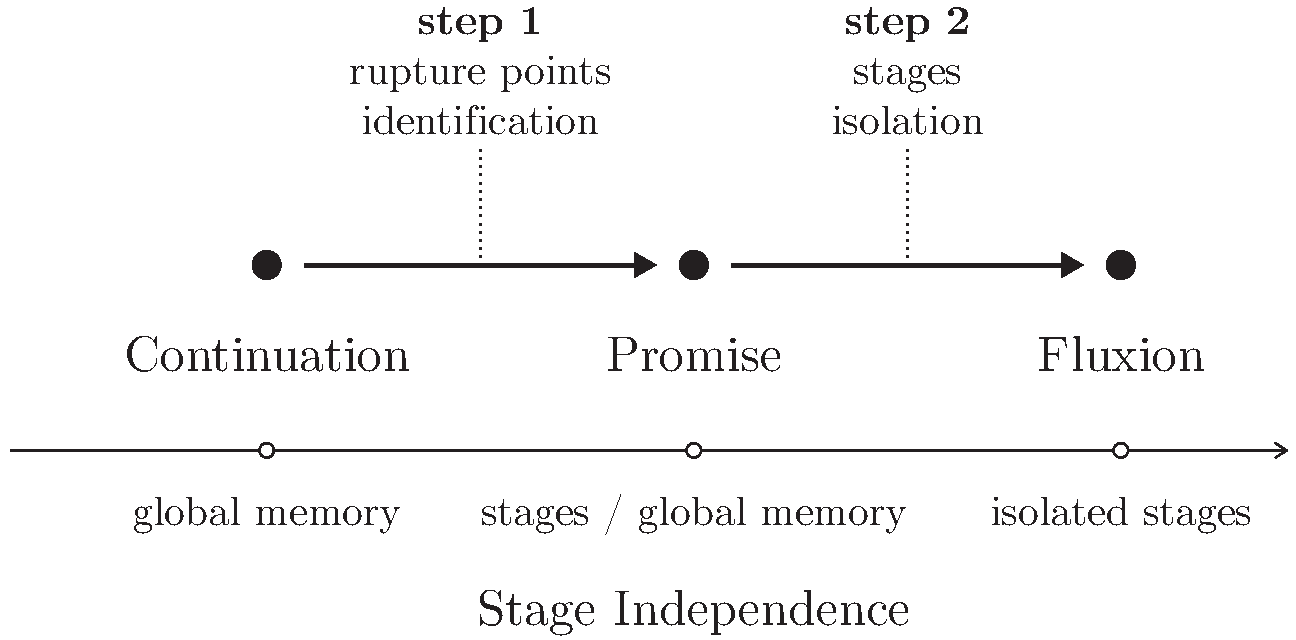
\includegraphics[width=0.9\textwidth]{../resources/roadmap.pdf}
\end{center}
\caption{Roadmap}
\label{fig:roadmap}
\end{figure}

\subsection{Rupture Point}

The pipeline architecture enforces the memory isolation between stages.
Each stage has its own thread of execution, and is independent from the others.
On the other hand, the execution flow of the event-loop jumps from one concurrent task to the other.
%  because of the continuation passing style and the common memory store.
% The message passing linking the callbacks is transparently handled by the event-loop.
However, the executions of these tasks are as distinct as the execution of the different stages of a pipeline.
The call stacks of two concurrent tasks are distinct.
The asynchronous function call between the caller and its continuation represents the rupture between two call stacks.
It is a rupture point, and is equivalent to a data stream between two stages in the pipeline architecture.

Both the pipeline architecture and the event-loop present these rupture points.
The detection of rupture points allows to map a pipeline architecture onto the implementation following the event-loop model.
To allow the transformation from one to the other, this thesis studies the possibility to detect rupture points, and to distribute the global memory into the parts defined by these rupture points.

The detection of rupture points is addressed in chapter \ref{chapter5}.
It presents the extraction of a pipeline of concurent tasks from a Javascript application.
Such pipeline is similar to the one exposed by Promises.
% The chapter proposes a simpler alternative to the latter called Dues.
However, these concurent tasks still require a global memory.
They can't be executed in parallel.

\subsection{Invariance}

% This transformation is important on two points.
% The conservation of the invariance.
% The equivalence between the coordinations.

The global memory assures the total ordering of tasks, and requires sequentiality, while message passing assures causal ordering of tasks and allows parallelism.
The causal ordering of tasks, by opposition to total ordering, is sufficient to assure the correctness of the execution.
Therefore, to assure the correctness of the execution, the ordering allowd by the global memory is partially equivalent to message passing ordering.
And it is possible to transform the global memory coordination into message passing.
% Given that the tasks are independent and communicate by messages.

% This result was used by Lamport to prove the correctness of distributed systems.
Yet, to preserve the correctness as expressed by the developer, it is important to preserve the invariance.
The global memory needs not to be distributed into each of the stages of the pipeline, so that each stage have an exclusive access to its memory.

To assure the missing coordinations assured by the shared memory between the stages, the transformation should provide equivalent coordination with message passing.
The isolation and replacement of the global memory is addressed in chapter \ref{chapter6}, with the introduction of isolated containers called Fluxions.




% The invariance holds for the whole memory during the execution of each callback.
% As I explained in the previous section, this invariance is required to allow the concurrent execution of the different tasks.
% On the other hand, the invariance is explicit in the pipeline architecture, as all the stages have isolated memories.
% The coordination between these isolated process is made explicit by the developer through message passing.

% I argue that the state coordination between the callbacks requireing a global memory could be replaced by the message passing coordination used manually in the pipeline architecture.
% I argue that not all applications need concurrent access on the state, and therefore, need a shared memory.
% % Specifically, I argue that each state region remains roughly local to a stage during its modification.
% \nt{TODO review that, I don't know how to formulate these paragraphs. Identify the state and the data in the global memory.}

% \subsubsection{Transformation}

% This equivalence should allow the transformation of an event loop into several parallel processes communicating by messages.
% In this thesis, I study the static transformation of a program, but the equivalence should also hold for a dynamic transformation.
% I present the analyzis tools I developed to identify the state and the data from the global memory.